\section{Video Recognition}

\subsection{Bag of Words}
\begin{frame}{Naive Bag of Words}

		\begin{tikzpicture}
			\node (video) at (-1, 0) {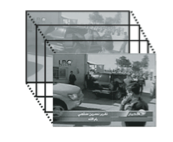
\includegraphics[scale=0.4]{videoSample.png}};
			\node (videoSIFT) at (2.5,0) {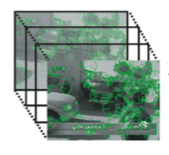
\includegraphics[scale=0.38]{videoSIFT.png}};

			\draw[->, line width = 2pt, black] (video) -- (videoSIFT) node[pos=.5, above] {\scriptsize{Locate}};

			\node (SIFTs) at (6,0) {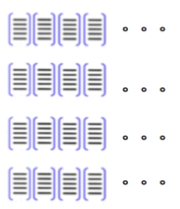
\includegraphics[scale=0.4]{SIFTs}};
			\draw[->, line width = 2pt, black] (videoSIFT) -- (SIFTs) node[pos=.5, above] {\scriptsize{Describe}};

			\node (his) at (9, 0) {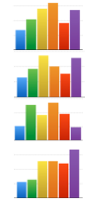
\includegraphics[scale=0.4]{his}};
			\draw[->, line width = 2pt, black] (SIFTs) -- (his) node[pos=.5, above] {\scriptsize{Project}};

		\end{tikzpicture}

		\begin{columns}
			\column{0.48\textwidth}
				\begin{itemize}
					\item $M$: number of sampled frames
					\item $V$: size of visual vocabulary 
				\end{itemize}
			\column{0.6\textwidth}

				\[
					  \left(\begin{array}{*5{c}}
					   	A_{11} & A_{12} & \cdots & \tikz[baseline]{\node[anchor=base] (t1) {$A_{1(V-1)}$};} & A_{1V}\\
						A_{21} & A_{22} & \cdots & A_{2(V-1)} & A_{2V}\\
						\vdots & \vdots & \vdots & \vdots & \vdots\\
						A_{M1} & A_{M2} & \cdots & A_{M(V-1)} & A_{MV}\\
					  \end{array}\right)
			    \]

	    \end{columns}

		\begin{tikzpicture}[overlay]

			\draw[->, line width = 2pt] (his) -- (t1); 

		\end{tikzpicture}
\end{frame}


\begin{frame}{Better Bag of Words - Soft Assignment}
	
	\begin{itemize}
		\item Straightforward approach \cite{jiang2007towards}
			\begin{itemize}
				\item Assign top $N$ nearest words to each feature
				\item Update the histogram by adding different weights to these $N$ words
			\end{itemize}

		\item Gaussian Mixture Models Assignment \cite{agarwal2006hyperfeatures} \\
			\vspace{2mm}
			\begin{tikzpicture}
				\node[draw, fill = gray!30] at (0,0) (trainVideo) {Training Videos};
				\node[draw, fill = gray!30] at (3.1,0) (SIFT) {SIFT Features};

				\node[draw, fill = gray!30] at (7,0) (GMM) {Gaussian Mixture Models};		


				\draw[->, line width = 2pt] (trainVideo) -- (SIFT);
				\draw[->, line width = 2pt] (SIFT) -- (GMM);



				\node (image) at (0,-2) {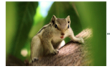
\includegraphics[scale=0.4]{image.png}};
				\node (oneSIFT) at (2.5,-2) {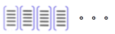
\includegraphics[scale=0.6]{oneSIFTs.png}};

				\draw[->, line width = 2pt] (image) -- (oneSIFT);

				\node[fill = green!30] (pro1) at (5.5, -1.5) {$[p_1, p_2, \cdots, p_K]$};
				\node[fill = green!30] (pro2) at (5.5, -2) {$[p_1, p_2, \cdots, p_K]$};
				\node (pro3) at (5.5, -2.5) {$\vdots$};
				\node[fill = green!30] (pro4) at (5.5, -3) {$[p_1, p_2, \cdots, p_K]$};

				\draw[->, line width = 2pt] (oneSIFT) -- (pro2) node[pos=.5,above] (middle){};
				\draw[->, line width = 2pt, red] (GMM) edge[bend right] (middle);

				\node (plus) at (7.2, -2.4) {$+$};
				\node[fill = red!30] (pro4) at (8.9, -2.4) {$[P_1, P_2, \cdots, P_K]$};

			\end{tikzpicture}
	\end{itemize}

\end{frame}


\begin{frame}{Better Bag of Words - Weighting Schemes \cite{yang2007evaluating}}
	\begin{itemize}
		\item Inverse document frequency of visual word $t_i$
				\begin{equation}
				idf(t_i) = \log(N / n_i)
				\end{equation}

				\begin{itemize}
					\item $N$ is the total number of images in the corpus
					\item $n_i$ is the number of images having visual word $t_i$
				\end{itemize}

		\item Various different weighting schemes
			
			\begin{table}[!ht]
	        \begin{center}

	        \scalebox{0.7}{
	          \begin{tabular}{ccc}
	          \hline
	          \head{Name} & \head{Factors} & \head{Value for $t_i$}\\
	          \hline
	    		bxx & $binary$ & 1 if $t_i$ presents, 0 if not \\
	    		txx & $tf$ & $tf_i$ \\
	    		txc & $tf, normalization$ & $\frac{tf_i}{\sum_i tf_i}$ \\
	    		tfx & $tf, idf$ & $tf_i \cdot \log(\sfrac{N}{n_i})$ \\
	    		tfc & $tf, idf, normalization$ & $ \frac{tf_i \cdot \log(\sfrac{N}{n_i})}{\sum_i tf_i \cdot \log(\sfrac{N}{n_i})}$ \\
	          \hline
	          \end{tabular}
	         }
	        \end{center}
	        \caption{Weighting schemes for visual-word feature \cite{yang2007evaluating}}
	    	\end{table}

	\end{itemize}
\end{frame}

\begin{frame}{Aligned Space-Time Pyramid Matching \cite{duan2012visual} at level 0}
\begin{itemize}
	\item Incorporate \alert{Earth Mover's Distance} (EMD) \cite{rubner2000earth}

	\item Given two videos $P$ and $Q$
	$$P = \{(p_1, 1 / m),...,(p_m, 1 / m) \}, Q = \{(q_1, 1 / n),...,(q_n, 1 / n) \}$$

	\item Solve the below optimization problem 
	\begin{columns}
		\column{0.6\textwidth}
			\begin{eqnarray}
			\text{minimize} & \sum_{i=1}^{m}\sum_{j=1}^{n}
			\tikz[baseline]{\node[fill=green!40,anchor=base] (t1)
			{$d_{ij}$};}\tikz[baseline]{\node[fill=red!40,anchor=base] (t2) {$f_{ij}$};} \nonumber \\
			\text{subjective to} & f_{ij} \geq 0 \quad \quad 1 \leq i \leq m,  1 \leq j \leq n \nonumber \\
			&\sum_{j=1}^n f_{ij} \leq 1 / m \quad 1 \leq i \leq m \nonumber \\
			&\sum_{i=1}^m f_{ij} \leq 1 / n \quad 1 \leq j \leq n\nonumber \\
			&\sum_{i=1}^{m} \sum_{j=1}^n f_{ij} = 1 
			\end{eqnarray}

		\column{0.4\textwidth}
			\begin{itemize}
				\item \tikz[na] \node[coordinate] (n1) {}; distance between $p_i$ and $q_j$
				\item \tikz[na] \node[coordinate] (n2) {}; flow between $p_i$ and $q_i$
			\end{itemize}

			\begin{figure}[!ht]
				\centering
					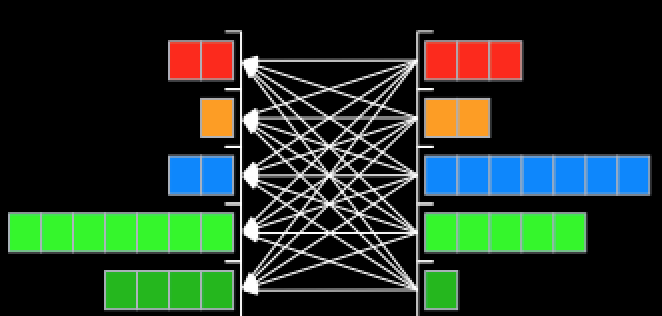
\includegraphics[scale=0.25]{./EMD.png}
				\end{figure}
	\end{columns}

	\begin{tikzpicture}[overlay]
		\path[->, green!40, line width = 2pt] (t1) edge [bend left] (n1); 
		\path[->, red!40, line width = 2pt] (t2) edge [bend left] (n2); 
	\end{tikzpicture}

	\item Distance between $P$ and $Q$
	\begin{equation}
	D_{PQ} = \frac{\sum_{i=1}^m \sum_{j=1}^n d_{ij} f_{ij}}{\sum_{i=1}^m\sum_{j=1}^n f_{ij}} 
	\end{equation}

\end{itemize}
\end{frame}


\begin{frame}{Aligned Space-Time Pyramid Matching \cite{duan2012visual} at level $l$}

	\begin{figure}[!ht]
	\centering
		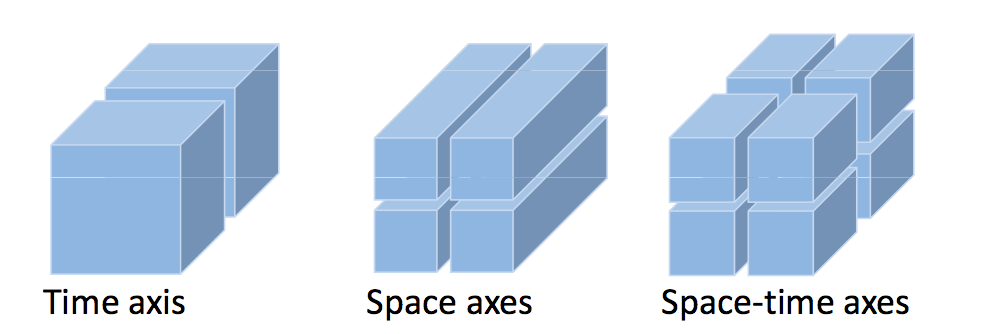
\includegraphics[scale=0.5]{./spaceTime.png}
	\end{figure}

\begin{itemize}
	\item Each video is divided into $8^l$ non-overlapped sub-videos
	\item Given two videos $P$ and $Q$
		$$P = (p_1, \cdots, p_R), Q = (q_1, \cdots, q_R), \text{where } R = 8^l$$
\end{itemize}
\end{frame}

\begin{frame}{Aligned Space-Time Pyramid Matching \cite{duan2012visual} at level $l$}

	\begin{figure}[!ht]
	\centering
		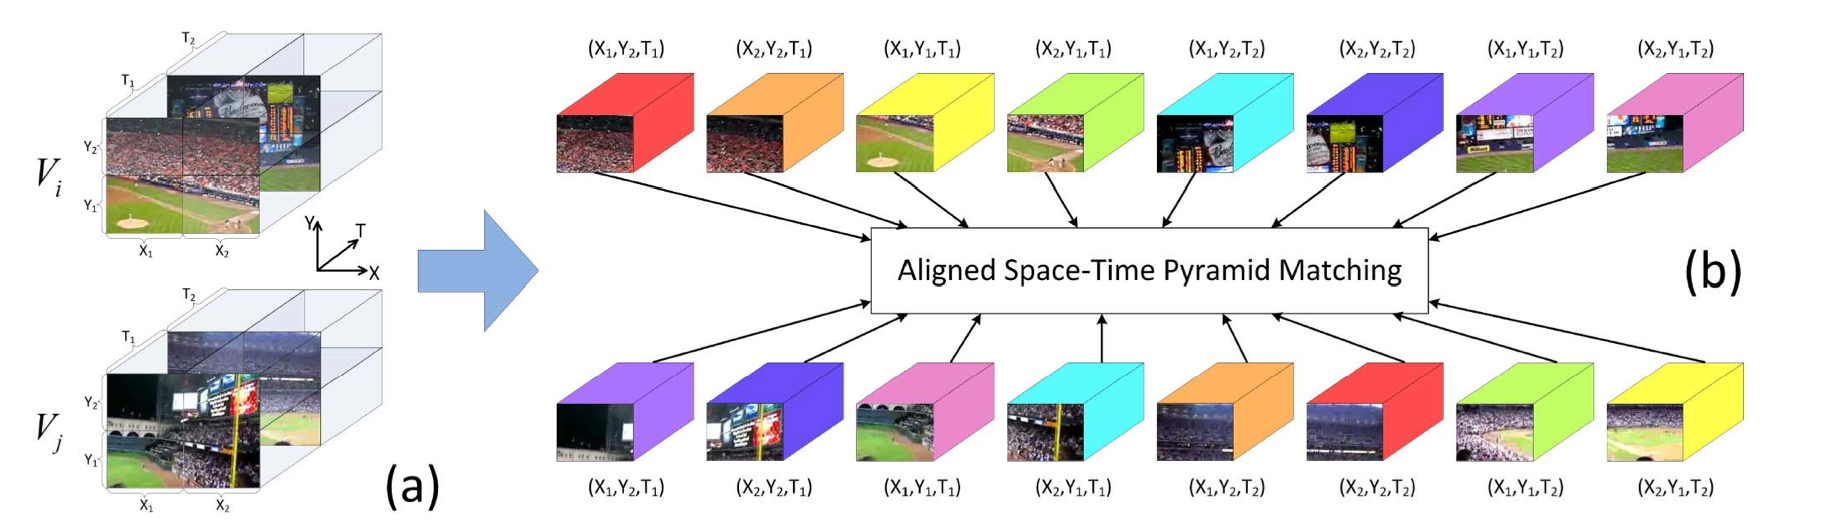
\includegraphics[scale=0.2]{./alignedST.png}
	\end{figure}


		\begin{enumerate}
			\item Calculate pairwise distance matrix $D$
				\begin{itemize}
					\item $D_{ij}$ is the EMD distance between sub-video $p_i$ and $q_i$
				\end{itemize}

			\item Align sub-videos in $P$ with sub-videos in $Q$ 
				\begin{eqnarray}
				& \hat F_{ij} = \argmin{F_{ij}} \sum_{i = 1}^{R} \sum_{j=1}^{R} F_{ij} D_{ij}
				\nonumber \\
				\text{subject to} & \sum_{i=1}^{R} F_{ij} = 1, \quad \forall j \nonumber\\
				&\sum_{j=1}^{R} F_{ij} = 1, \quad \forall i
				\end{eqnarray}

				\begin{equation}
				D_l(P,Q) = \frac{\sum_{i=1}^R \sum_{j=1}^R \hat F_{ij} D_{ij}}{\sum_{i=1}^R \sum_{j=1}^R F_{ij}}
				\end{equation}
		\end{enumerate}


\end{frame}

\begin{frame}{Experiments of Aligned Space-Time Pyramid Matching}
	
	\begin{itemize}
		\item Data set
			\begin{table}[!ht]
			\begin{center}
			\scalebox{0.7}{
			\begin{tabular}{cccccccc}
			\hline
			\head{} & \head{Wedding} & \head{Sports} & \head{Show} & \head{Picnic} & \head{Parade} & \head{Birthday} & \head{Total}\\
			\hline
			Kodak & 27 & 75 & 57 & 6 & 14 & 16 & 195\\   
			\hline
			\end{tabular}
			}
			\end{center}
			\caption{Number of videos in each class from Kodak }
			\end{table}
		\item Kernel types
			\begin{columns}
				\column{0.4\textwidth}
					\begin{table}[!ht]
					    \begin{center}
					      \scalebox{0.75}{
					      \begin{tabular}{cc}
					      \hline
					      \head{Kernel type} & \head{Kernel function}\\
					      \hline
					      Gaussian & $\exp(-\gamma D^2(I_i, I_j)$ \\
					      Laplacian & $\exp(- \sqrt{\gamma} D(I_i, I_j)$ \\
					      ISD & $\frac{1}{\gamma D^2(I_i, I_j) + 1}$ \\
					      ID & $\frac{1}{\sqrt{\gamma}D(I_i, I_j) + 1}$\\
					      \hline
					      \end{tabular}
					      }
					    \end{center}
					\end{table}

				\column{0.6\textwidth}
					\begin{itemize}
						\item $D(I_i, I_j)$ represents the distance between $I_i$ and $I_j$
						\item $\gamma = \frac{1}{A}$, $A$ is the mean value of the squared distances between training samples

						\item \alert{Fused scores}
						\begin{equation}
						f^{Fuse} = \frac{1}{N} \sum_{i=1}^{N} \frac{1}{1 +\exp{(-f_i)}}
						\end{equation} 
					\end{itemize}
			\end{columns}
	\end{itemize}		
\end{frame}

\begin{frame}{Experiments of Aligned Space-Time Pyramid Matching}
	\begin{itemize}
			\item Division of training and testing samples
			\begin{itemize}
				\item randomly select 3 videos from each class as training samples
				\item the rest of videos act as testing samples
			\end{itemize}

			\item Evaluation metric: Mean Average Precision

			\item Experimental results at different levels using histograms built by naive bag of words

				\begin{table}[!ht]
				\begin{center}
				\scalebox{0.7}{
				\begin{tabular} {cccccc}
				\hline
				\head{} & \head{Gaussian} & \head{Laplacian} & \head{ISD} & \head{ID} &\head{Fused scores}\\
				\hline
				Level 0 & $44.38 \pm 2.13$ & $44.90 \pm 2.73$ & $44.01 \pm 2.13$ & $45.36 \pm 3.13$ & $44.33 \pm 2.61$ \\
				Level 1 (Unaligned) &$43.08 \pm 3.14$ &$43.85\pm3.84$ &$43.22\pm3.11$ &$43.85\pm3.56$ &$43.55\pm3.46$ \\
				Level 1 (Aligned)&$43.61\pm2.97$ &$43.40\pm3.18$ &$43.46\pm2.97$ &$43.22\pm3.11$ & $44.08\pm3.25$ \\
				  \hline
				  \end{tabular}
				  }
				\end{center}
				\caption{Means and standard deviations (percent) of MAPs at different levels}
				\end{table}
	\end{itemize}
\end{frame}

\begin{frame}{Experiments of Aligned Space-Time Pyramid Matching}
	\begin{itemize}
		\item Experimental results using histograms built by better bag of words at level $0$ distance
		\begin{table}[!ht]
		\begin{center}
		\scalebox{0.7}{
		\begin{tabular} {cccccc}
		\hline
		\head{} & \head{Gaussian} & \head{Laplacian} & \head{ISD} & \head{ID} &\head{Fused scores}\\
		\hline
		bxx& $40.20 \pm 2.57$ & $38.35 \pm 2.31$ & $39.93 \pm 2.58$ & $38.23 \pm 2.08$ & $39.34 \pm 2.55$ \\
		txx& $44.28 \pm 2.14$ & $44.90 \pm 2.73$ & $44.01 \pm 2.13 $ & $45.36 \pm 3.13 $ & $44.33 \pm 2.61$ \\
		txc& $ 42.15 \pm 4.73$ & $45.01 \pm 3.45$ & $43.47 \pm 4.56$ & $45.38 \pm 3.20$ & $44.11 \pm 3.90$ \\
		tfx& $ 43.76 \pm 2.99$ & $44.14 \pm 3.36$ & $43.61 \pm 3.03$ & $44.05 \pm 3.51$ & $44.18 \pm 3.22$ \\

		\alert{tfc}& $ 43.71\pm 1.37$ & $\mathbf{46.02 \pm 1.84}$ & $\mathbf{44.93 \pm 1.64}$ & $\alert{\mathbf{46.21 \pm 1.83}}$ & $\mathbf{45.28 \pm 1.62}$ \\
		Easy soft& $43.54 \pm 2.12$ & $ 44.77\pm 2.41$ & $43.52 \pm 2.08$ & $45.24 \pm 2.47$ & $ 44.79\pm 2.55$ \\
		\alert{Gaussian soft}& $\mathbf{44.77 \pm 2.80}$ & $45.23 \pm 2.76$ & $44.90 \pm 3.01$ & $45.23 \pm 2.87$ & $\mathbf{45.20 \pm 3.04}$ \\
		\hline
		\end{tabular}
		}
		\end{center}
		\caption{Means and standard deviations (percent) of MAPs using different mechanisms to build histograms at level 0}
		\end{table}
	\end{itemize}
\end{frame}


\subsection{Gaussian Mixture Models}
\begin{frame}{Gaussian Mixture Models to Represent Videos \cite{zhou2008sift}}

\begin{columns}
	\column{0.5\textwidth}
			\begin{figure}[!ht]
				\centering
					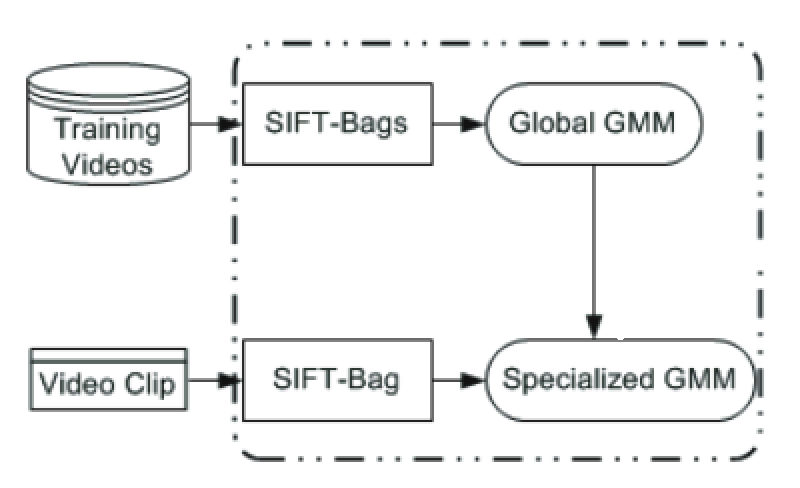
\includegraphics[scale=0.2]{./gmm.png}
				\end{figure}		

	\column{0.6\textwidth}
		\begin{itemize}
			\item Global GMM built from training data
			\item Specialized GMM by adaption
		\end{itemize}
\end{columns}

\begin{itemize}
	\item Specialized GMM of video $P$ and $Q$
		$$P = (\mu_1^p, \cdots, \mu_K^p), Q = (\mu_1^q, \cdots, \mu_K^q)$$
	\item Given global GMM as $\Theta = \{w_1, \mu_1, \Sigma_1, \cdots\}$, the distance of $P$ and $Q$
	\begin{equation}
	d(P,Q) = \frac{1}{2} \sum_{k= 1}^{K} w_k (\mu_k^p - \mu_k^q)^T \Sigma_k^{-1} (\mu_k^p - \mu_k^q)
	\end{equation}
\end{itemize}

\end{frame}

\begin{frame}{Experiments on GMM}

\begin{table}[!ht]
  \begin{center}
  \scalebox{0.7}{
    \begin{tabular} {cccccc}
    \hline
    \head{} & \head{Gaussian} & \head{Laplacian} & \head{ISD} & \head{ID} &\head{Fused scores}\\
    \hline
    spherical 128& $24.70 \pm 1.41 $ & $ 43.04 \pm 1.61 $ & $26.92 \pm 1.00$ & $\alert{\mathbf{43.64 \pm 0.96}}$ & $ 32.91 \pm 2.20$ \\
    spherical 64& $ 23.99 \pm 1.40$ & $42.35 \pm 1.64$ & $ 25.62\pm 1.11$ & $43.42 \pm 1.18$ & $29.01 \pm 1.10$ \\
    full 128& $ 25.69 \pm 7.57 $ & $21.39 \pm 7.32$ & $26.49 \pm 8.38$ & $21.93 \pm 7.75$ & $21.79 \pm 7.29$ \\
    full 64& $  25.23 \pm 0.94$ & $ 29.69 \pm 1.81$ & $25.68 \pm 1.34$ & $30.74 \pm 1.67$ & $26.74 \pm 1.63$ \\
    \hline
    \end{tabular}
    }
    \end{center}
    \caption{Means and standard deviations (percent) of MAPs using different GMMs}
\end{table}

\begin{itemize}
	\item Spherical covariance using ID kernel performed the best
	\item Spherical covariance performed better than full covariance
\end{itemize}
\end{frame}

\subsection{Concept Attributes}
\begin{frame}{Concept Attributes to Represent Videos \cite{liu2013video}}
		\begin{tikzpicture}
			
			\node[draw, fill = gray!30] (trainVideos) at (2, 2.7) {Training Videos};

			\node[fill = green!20] (clf1) at (4,1) {classifier $1$};
			\node[fill = green!20] (clf2) at (4,0.2) {classifier $2$};
			\node[] (clf3) at (4,-0.5) {$\vdots$};
			\node[fill = green!20] (clf4) at (4,-1.3) {classifier $n$};

			\draw[black,thick,dotted] ($(clf1.north west)+(-0.2,0.3)$)  rectangle ($(clf4.south east)+(0.2,-0.3)$);

			\draw[->, line width = 2pt] (trainVideos) -- ($(clf1.north)+(0,0.3)$) node[pos= 0.6, above] {\scriptsize{Train}};

			\node (video) at (0, 0) {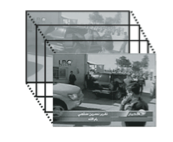
\includegraphics[scale=0.4]{videoSample.png}};
			\draw[->, line width = 2pt] (video) -- ($(clf2.west)+(-0.3, -0.2)$) node[pos=.5, above] {Input};

			\node[fill = red!20] (ca) at (7, 0) {$[c_1, c_2, \cdots, c_n]$};
			\draw[->, line width = 2pt] ($(clf2.east)+(0.2, -0.2)$) -- (ca);

			\node(c) at (7, -1) {\small{Concept Attributes}};


			\node[draw, fill = gray!30] (svm) at (10, 0) {SVM};
			\draw[->, line width = 2pt] (ca) -- (svm) node[pos=0.5, above] {\scriptsize{Classify}};
		\end{tikzpicture}

			\begin{enumerate}
				\item Recognize complex events
				\item Make use of pre-trained detectors (even by others)
			\end{enumerate}

\end{frame}

\begin{frame}{Experiments on Concept Attributes}

	  \begin{table}[!ht]
    \begin{center}
    \scalebox{0.7}{
      \begin{tabular}{cccccccc}
      \hline
      \head{} & \head{Wedding} & \head{Sports} & \head{Show} & \head{Picnic} & \head{Parade} & \head{Birthday} & \head{Total}\\
      \hline
      Kodak & 27 & 75 & 57 & 6 & 14 & 16 & 195\\
      Youtube & 91 & 260 & 200 & 85 & 119 & 151 & 906\\
      \hline
      \end{tabular}
    }
    \end{center}
    \caption{Number of videos in each class from Kodak and Youtube}
  \end{table}

	\begin{table}[!ht]
	  \begin{center}
    \scalebox{0.7}{
	    \begin{tabular} {cc}
	    \hline
	    \head{} & \head{Recognition Accuracy}\\
	    \hline
	    Kodak $\to$ Kodak & $38.5 \pm 12.7$\\
	    Youtube $\to$ Kodak & $30.0 \pm 6.9$\\
	    Baseline & $41.6 \pm 11.5$\\
	    \hline
	    \end{tabular}
		}
	    \end{center}
	    \caption{Means and standard deviations (percent) of recognition accuracies}
	\end{table}

\end{frame}

\subsection{Compressed Videos}
\begin{frame}{Compress Videos}

	\begin{enumerate}
		\item Run K-Means on sampled frames of a video
		\item Build a graph for each cluster
		\item Choose representative frames from each graph
	\end{enumerate}

			\begin{figure}[!ht]
				\centering
				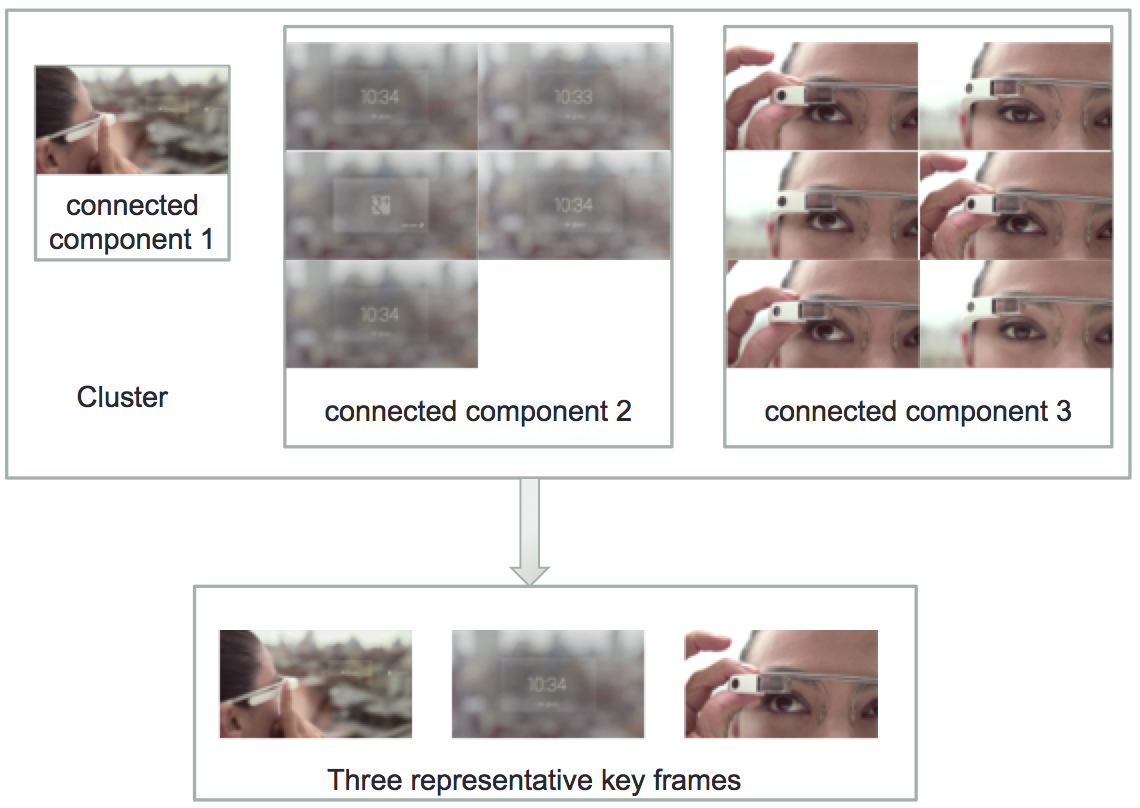
\includegraphics[scale=0.32]{./keyFrames.png}
			\end{figure}
\end{frame}

\begin{frame}{Experiments on Compressed Videos}

\begin{itemize}
	\item Size of Youtube videos is compressed from 4.42 GB to 3.17 GB. ($28.41 \%$ reduced)
	
	\vspace{5mm}
	\begin{table}[!ht]
  	\begin{center}
  	\scalebox{0.7}{
    \begin{tabular} {cccc}
    \hline
    \head{Training videos} & \head{Testing videos} &\head{Original videos} &\head{Compressed videos}\\
    \hline
    60 & 846 &  $38.9 \pm 2.9$  & $38.6 \pm 2.8$ \\
    120 & 786 & $45.7 \pm 2.2$  & $44.5 \pm 1.6$ \\
    180 & 726 & $49.5 \pm 1.8$  & $48.3 \pm 1.9$ \\
    240 & 666 & $52.0 \pm 2.1$  & $50.6 \pm 2.1$\\
    \hline
    \end{tabular}
    }
    \end{center}
    \caption{Means and standard deviations (percent) of MAPs over six events}
	\end{table}
\end{itemize}
		
	\begin{enumerate}	
		\item Compressed videos performed slightly worse than original videos
		\item With more training samples, the performance increases
	\end{enumerate}

\end{frame}